 \documentclass[student, noshadow, lsr, english, aspectratio=169]{ITR_LSR_slides}
% student options:
% lsr 				-> lsr, template (remove for itr)
% english 			-> enables english language format
% aspectratio=43	-> 4:3 layout
\usepackage{tikz}
\usepackage{pgfplots}
\pgfdeclarelayer{background}
\pgfdeclarelayer{nodelayer}
\pgfdeclarelayer{edgelayer}
\pgfdeclarelayer{foreground}
\pgfsetlayers{background,edgelayer,nodelayer,main,foreground}
\tikzset{robotRec/.style={rectangle, draw=black,line width=2.5pt, fill=tum_gray, rounded corners=9pt, minimum width=60pt, minimum height=30pt}}
\tikzset{robotCirc/.style={circle, draw=black, fill=black, line width=1.5pt}}
% robot name for tikz figure
\newcommand{\RobotName}{$\mathbf{R}$}
\addbibresource{ref.bib}
\graphicspath{{pics/}{logos/}}

\title{Titel der Präsentation}
\presenter{S. Student}

\supervisor{B. Betreuer}
\typeofpres{Zwischenbericht Masterarbeit}

\usepackage[bigfiles]{media9} %option bigfiles not needed for xelatex, runs without problems on ubuntu14
%%%%%%%%%%%%%%%%%%%%%%%%%%%%%%%%%%%%%%%%%%%%%%%%%%%%%%%%%%%%%%%%%%%%%%%%%%%%%%%%

\begin{document}


\begin{frame}
    \titlepage
\end{frame}


\section{Einführung}

\begin{frame}
	\frametitle{Einführung1}
	\begin{itemize}
 		\item $y=x^2+\sqrt{z}+\int_{a}^{b}{xyz}$
	\end{itemize}
\end{frame}

\begin{frame}
	\frametitle{Einführung2}

% EPS tutorial
%\begin{figure}[htb]
%\centering
%\psfrag{q1}[Bl][Bl]{\small $\alpha$}
%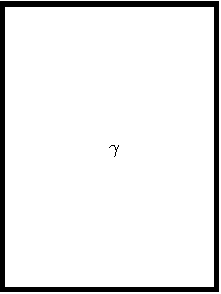
\includegraphics[width=0.9\textwidth]{samplefigure.eps}
%\caption{Sample Figure}
%\end{figure}

\end{frame}

\begin{frame}
	\frametitle{Related Work}
    Normal cite: \cite{buss11}\\
	Bigger cite: \scite{buss11}\\
	Multiple  authors: \cite[3]{bauer09}
\end{frame}

\section{Methoden}

\begin{frame}
	\frametitle{Methoden1}
	\begin{itemize}
		\item a
		\item b
	\end{itemize}
\end{frame}

\begin{frame}
	\frametitle{Methoden2}
	\begin{itemize}
		\item a
	\end{itemize}
\end{frame}

\begin{frame}
	\frametitle{Methoden3}
	\begin{itemize}
		\item a
	\end{itemize}
\end{frame}

\section{Ergebnisse}

\begin{frame}
	\frametitle{Ergebnisse1}
	...
\end{frame}

\begin{frame}
	\frametitle{Ergebnisse2}
	...
\end{frame}

%%%%%%%%%%%%%%%%%%%%%%%%%%%%%%%%%%%%%%%%%%%%%%%%%%%%%%%%%%%%%%%%%%%%%%%%%%%%%%%%%%%%%%%%%%%%%%%%%%%%%%%%%%%%%%%%%%%%%%%%%%%%%%%%%%%%%%%%%%%%%
% VIDEO: both examples below show a figure where the video will be displayed. 
% This figure could be a still picture of the video, giving a hint on what the video will show. 
% Usage of such a figure can be useful in case the presentation is likely to be printed as e.g. a handout 
% Please comment in slides shown below yourself for testing!
% NOTE: the folder containing the videos MUST BE INSIDE the presentation folder, otherwise the videos might not show up in the presentation.
% Also: the videos cannot be displayed on ubuntu, use e.g. the windows imperator to check whether the videos work

%video example1
% comment out manually
%{
%    \usebackgroundtemplate{\includemedia[width=12.8cm,height=9.6cm,activate=onclick,]{
\includegraphics{motivation}}{movie/example_video_short.swf}} 
%    \begin{frame}[plain]
%    \end{frame}
%}

%video example2
% \begin{frame}
% 	\frametitle{Example video}
% \includemedia[height=.5\textwidth]{
\includegraphics[height=.5\textwidth]{motivation}}{movie/example_video_short.swf} 
% \end{frame}
%%%%%%%%%%%%%%%%%%%%%%%%%%%%%%%%%%%%%%%%%%%%%%%%%%%%%%%%%%%%%%%%%%%%%%%%%%%%%%%%%%%%%%%%%%%%%%%%%%%%%%%%%%%%%%%%%%%%%%%%%%%%%%%%%%%%%%%%%%%%%%%%
\section{Zusammenfassung}

\begin{frame}
	\frametitle{Zusammenfassung}
	...
\end{frame}

\appendix

\begin{frame}[plain]
	% This slide serves 3 purposes:
	% 	1. a simple example how to create figures in tikz using beamer
	%	2. testing if you actually checked the content of this template
	% 	3. subtly preventing you from adding a "Thank you..." slide at the end of your presentation
	% If this slide is still in your final presentation... well, congratulation!
	\begin{center}
		{\fontsize{40}{50} \structure{Sorry for your attention\\}}
		\renewcommand{\RobotName}{I}
		\resizebox {!} {0.16\textwidth} {\begin{tikzpicture}
	% nodes
	\begin{pgfonlayer}{nodelayer}
		\node (roboHead) {
			\begin{tikzpicture}
% nodes
\begin{pgfonlayer}{nodelayer}
	\node[robotRec](head){};
	\node[robotCirc, fill=white, minimum size=2pt, above=2pt of head.north](antennaBulb){};
	\node[robotCirc, fill=white, minimum size=7pt](eyeL)at ($(head.135)!0.4!(head.225)$){};
	\node[robotCirc, minimum size=1pt,scale=0.3](eyeLMid) at ($(head.135)!0.4!(head.225)$){};
	\node[robotCirc, fill=white, minimum size=7pt](eyeR) at ($(head.45) !0.4!(head.315)$){};
	\node[robotCirc, minimum size=1pt,scale=0.3](eyeRMid) at ($(head.45) !0.4!(head.315)$){};
\end{pgfonlayer}

% coordinate helpers
\coordinate (mouth1)  at ($(head.130)!0.73!(head.230)$);
\coordinate (mouth2)  at ($(head.50)!0.73!(head.310)$);
\coordinate (tongue)  at ($(mouth1)!0.88!(mouth2)$);

% edges (behind node layer)
\begin{pgfonlayer}{edgelayer}
	\draw[line width=3pt] (head.center) --  (antennaBulb.center) ;
\end{pgfonlayer}

% edges in foreground
\begin{pgfonlayer}{foreground}
	\draw[line width=2pt,line cap=round] (mouth1) --  (mouth2);
	\draw[line width=1.5pt] (tongue) arc[draw, start angle=0, end angle=-180, x radius=4pt, y radius=3pt];
\end{pgfonlayer}
\end{tikzpicture}
		};	
		\node[robotRec, minimum height=40pt, below=1pt of roboHead, anchor=north](body){\Large\RobotName};
		%feet
		\node[robotRec, minimum width=30pt, rounded corners=4pt, minimum height=10pt, below left = 2pt and -12pt of body, anchor=north](footL){};
		\node[robotRec, minimum width=30pt, rounded corners=4pt, minimum height=10pt, below right = 2pt and -12pt of body,anchor=north](footR){};
		\node[robotRec, minimum width=10pt, rounded corners=4pt, minimum height=30pt, below left = 2.5pt and -5pt of body.north west,anchor=north,rotate=-40](armL){};
		\node[robotRec, minimum width=10pt, rounded corners=4pt, minimum height=30pt, below right = 2pt and -1pt of body.north east,anchor=north](armR){};
	\end{pgfonlayer}
	
	% nodes in background 
	\begin{pgfonlayer}{background}	
		\node[robotRec, minimum width=15pt, rounded corners=2pt, minimum height=20pt, above=10pt of roboHead.south, anchor=north](neck){};
		\node[robotRec, minimum width=15pt, rounded corners=2pt, minimum height=20pt, above=10pt of footL.north, 	anchor=north](legL){};
		\node[robotRec, minimum width=15pt, rounded corners=2pt, minimum height=20pt, above=10pt of footR.north, anchor=north](legR){};
	\end{pgfonlayer}
	
	% coordinates
	\coordinate (handLCon)  at ($(armL.south)+(0pt,-9pt)$);
	\coordinate (handRCon)  at ($(armR.south)+(8pt,-8pt)$);
		
	% edges
	\begin{pgfonlayer}{foreground}
		\draw[line width=3pt,line cap=round] (handLCon) arc[draw, start angle=-40, end angle=145, x radius=8pt, y radius=8pt];
		\draw[line width=3pt,line cap=round] (handRCon) arc[draw, start angle=0, end angle=180, x radius=8pt, y radius=8pt];
	\end{pgfonlayer}
\end{tikzpicture}}
		\renewcommand{\RobotName}{DID}
		\resizebox {!} {0.16\textwidth} {\begin{tikzpicture}
	% nodes
	\begin{pgfonlayer}{nodelayer}
		\node (roboHead) {
			\begin{tikzpicture}
% nodes
\begin{pgfonlayer}{nodelayer}
	\node[robotRec](head){};
	\node[robotCirc, fill=white, minimum size=2pt, above=2pt of head.north](antennaBulb){};
	\node[robotCirc, fill=white, minimum size=7pt](eyeL)at ($(head.135)!0.4!(head.225)$){};
	\node[robotCirc, minimum size=1pt,scale=0.3](eyeLMid) at ($(head.135)!0.4!(head.225)$){};
	\node[robotCirc, fill=white, minimum size=7pt](eyeR) at ($(head.45) !0.4!(head.315)$){};
	\node[robotCirc, minimum size=1pt,scale=0.3](eyeRMid) at ($(head.45) !0.4!(head.315)$){};
\end{pgfonlayer}

% coordinate helpers
\coordinate (mouth1)  at ($(head.130)!0.73!(head.230)$);
\coordinate (mouth2)  at ($(head.50)!0.73!(head.310)$);
\coordinate (tongue)  at ($(mouth1)!0.88!(mouth2)$);

% edges (behind node layer)
\begin{pgfonlayer}{edgelayer}
	\draw[line width=3pt] (head.center) --  (antennaBulb.center) ;
\end{pgfonlayer}

% edges in foreground
\begin{pgfonlayer}{foreground}
	\draw[line width=2pt,line cap=round] (mouth1) --  (mouth2);
	\draw[line width=1.5pt] (tongue) arc[draw, start angle=0, end angle=-180, x radius=4pt, y radius=3pt];
\end{pgfonlayer}
\end{tikzpicture}
		};	
		\node[robotRec, minimum height=40pt, below=1pt of roboHead, anchor=north](body){\Large\RobotName};
		%feet
		\node[robotRec, minimum width=30pt, rounded corners=4pt, minimum height=10pt, below left = 2pt and -12pt of body, anchor=north](footL){};
		\node[robotRec, minimum width=30pt, rounded corners=4pt, minimum height=10pt, below right = 2pt and -12pt of body,anchor=north](footR){};
		\node[robotRec, minimum width=10pt, rounded corners=4pt, minimum height=30pt, below left = 2.5pt and -5pt of body.north west,anchor=north,rotate=-40](armL){};
		\node[robotRec, minimum width=10pt, rounded corners=4pt, minimum height=30pt, below right = 2pt and -1pt of body.north east,anchor=north](armR){};
	\end{pgfonlayer}
	
	% nodes in background 
	\begin{pgfonlayer}{background}	
		\node[robotRec, minimum width=15pt, rounded corners=2pt, minimum height=20pt, above=10pt of roboHead.south, anchor=north](neck){};
		\node[robotRec, minimum width=15pt, rounded corners=2pt, minimum height=20pt, above=10pt of footL.north, 	anchor=north](legL){};
		\node[robotRec, minimum width=15pt, rounded corners=2pt, minimum height=20pt, above=10pt of footR.north, anchor=north](legR){};
	\end{pgfonlayer}
	
	% coordinates
	\coordinate (handLCon)  at ($(armL.south)+(0pt,-9pt)$);
	\coordinate (handRCon)  at ($(armR.south)+(8pt,-8pt)$);
		
	% edges
	\begin{pgfonlayer}{foreground}
		\draw[line width=3pt,line cap=round] (handLCon) arc[draw, start angle=-40, end angle=145, x radius=8pt, y radius=8pt];
		\draw[line width=3pt,line cap=round] (handRCon) arc[draw, start angle=0, end angle=180, x radius=8pt, y radius=8pt];
	\end{pgfonlayer}
\end{tikzpicture}}
		\renewcommand{\RobotName}{NOT}
		\resizebox {!} {0.16\textwidth} {\begin{tikzpicture}
	% nodes
	\begin{pgfonlayer}{nodelayer}
		\node (roboHead) {
			\begin{tikzpicture}
% nodes
\begin{pgfonlayer}{nodelayer}
	\node[robotRec](head){};
	\node[robotCirc, fill=white, minimum size=2pt, above=2pt of head.north](antennaBulb){};
	\node[robotCirc, fill=white, minimum size=7pt](eyeL)at ($(head.135)!0.4!(head.225)$){};
	\node[robotCirc, minimum size=1pt,scale=0.3](eyeLMid) at ($(head.135)!0.4!(head.225)$){};
	\node[robotCirc, fill=white, minimum size=7pt](eyeR) at ($(head.45) !0.4!(head.315)$){};
	\node[robotCirc, minimum size=1pt,scale=0.3](eyeRMid) at ($(head.45) !0.4!(head.315)$){};
\end{pgfonlayer}

% coordinate helpers
\coordinate (mouth1)  at ($(head.130)!0.73!(head.230)$);
\coordinate (mouth2)  at ($(head.50)!0.73!(head.310)$);
\coordinate (tongue)  at ($(mouth1)!0.88!(mouth2)$);

% edges (behind node layer)
\begin{pgfonlayer}{edgelayer}
	\draw[line width=3pt] (head.center) --  (antennaBulb.center) ;
\end{pgfonlayer}

% edges in foreground
\begin{pgfonlayer}{foreground}
	\draw[line width=2pt,line cap=round] (mouth1) --  (mouth2);
	\draw[line width=1.5pt] (tongue) arc[draw, start angle=0, end angle=-180, x radius=4pt, y radius=3pt];
\end{pgfonlayer}
\end{tikzpicture}
		};	
		\node[robotRec, minimum height=40pt, below=1pt of roboHead, anchor=north](body){\Large\RobotName};
		%feet
		\node[robotRec, minimum width=30pt, rounded corners=4pt, minimum height=10pt, below left = 2pt and -12pt of body, anchor=north](footL){};
		\node[robotRec, minimum width=30pt, rounded corners=4pt, minimum height=10pt, below right = 2pt and -12pt of body,anchor=north](footR){};
		\node[robotRec, minimum width=10pt, rounded corners=4pt, minimum height=30pt, below left = 2.5pt and -5pt of body.north west,anchor=north,rotate=-40](armL){};
		\node[robotRec, minimum width=10pt, rounded corners=4pt, minimum height=30pt, below right = 2pt and -1pt of body.north east,anchor=north](armR){};
	\end{pgfonlayer}
	
	% nodes in background 
	\begin{pgfonlayer}{background}	
		\node[robotRec, minimum width=15pt, rounded corners=2pt, minimum height=20pt, above=10pt of roboHead.south, anchor=north](neck){};
		\node[robotRec, minimum width=15pt, rounded corners=2pt, minimum height=20pt, above=10pt of footL.north, 	anchor=north](legL){};
		\node[robotRec, minimum width=15pt, rounded corners=2pt, minimum height=20pt, above=10pt of footR.north, anchor=north](legR){};
	\end{pgfonlayer}
	
	% coordinates
	\coordinate (handLCon)  at ($(armL.south)+(0pt,-9pt)$);
	\coordinate (handRCon)  at ($(armR.south)+(8pt,-8pt)$);
		
	% edges
	\begin{pgfonlayer}{foreground}
		\draw[line width=3pt,line cap=round] (handLCon) arc[draw, start angle=-40, end angle=145, x radius=8pt, y radius=8pt];
		\draw[line width=3pt,line cap=round] (handRCon) arc[draw, start angle=0, end angle=180, x radius=8pt, y radius=8pt];
	\end{pgfonlayer}
\end{tikzpicture}}
		\renewcommand{\RobotName}{CHECK}
		\resizebox {!} {0.16\textwidth} {\begin{tikzpicture}
	% nodes
	\begin{pgfonlayer}{nodelayer}
		\node (roboHead) {
			\begin{tikzpicture}
% nodes
\begin{pgfonlayer}{nodelayer}
	\node[robotRec](head){};
	\node[robotCirc, fill=white, minimum size=2pt, above=2pt of head.north](antennaBulb){};
	\node[robotCirc, fill=white, minimum size=7pt](eyeL)at ($(head.135)!0.4!(head.225)$){};
	\node[robotCirc, minimum size=1pt,scale=0.3](eyeLMid) at ($(head.135)!0.4!(head.225)$){};
	\node[robotCirc, fill=white, minimum size=7pt](eyeR) at ($(head.45) !0.4!(head.315)$){};
	\node[robotCirc, minimum size=1pt,scale=0.3](eyeRMid) at ($(head.45) !0.4!(head.315)$){};
\end{pgfonlayer}

% coordinate helpers
\coordinate (mouth1)  at ($(head.130)!0.73!(head.230)$);
\coordinate (mouth2)  at ($(head.50)!0.73!(head.310)$);
\coordinate (tongue)  at ($(mouth1)!0.88!(mouth2)$);

% edges (behind node layer)
\begin{pgfonlayer}{edgelayer}
	\draw[line width=3pt] (head.center) --  (antennaBulb.center) ;
\end{pgfonlayer}

% edges in foreground
\begin{pgfonlayer}{foreground}
	\draw[line width=2pt,line cap=round] (mouth1) --  (mouth2);
	\draw[line width=1.5pt] (tongue) arc[draw, start angle=0, end angle=-180, x radius=4pt, y radius=3pt];
\end{pgfonlayer}
\end{tikzpicture}
		};	
		\node[robotRec, minimum height=40pt, below=1pt of roboHead, anchor=north](body){\Large\RobotName};
		%feet
		\node[robotRec, minimum width=30pt, rounded corners=4pt, minimum height=10pt, below left = 2pt and -12pt of body, anchor=north](footL){};
		\node[robotRec, minimum width=30pt, rounded corners=4pt, minimum height=10pt, below right = 2pt and -12pt of body,anchor=north](footR){};
		\node[robotRec, minimum width=10pt, rounded corners=4pt, minimum height=30pt, below left = 2.5pt and -5pt of body.north west,anchor=north,rotate=-40](armL){};
		\node[robotRec, minimum width=10pt, rounded corners=4pt, minimum height=30pt, below right = 2pt and -1pt of body.north east,anchor=north](armR){};
	\end{pgfonlayer}
	
	% nodes in background 
	\begin{pgfonlayer}{background}	
		\node[robotRec, minimum width=15pt, rounded corners=2pt, minimum height=20pt, above=10pt of roboHead.south, anchor=north](neck){};
		\node[robotRec, minimum width=15pt, rounded corners=2pt, minimum height=20pt, above=10pt of footL.north, 	anchor=north](legL){};
		\node[robotRec, minimum width=15pt, rounded corners=2pt, minimum height=20pt, above=10pt of footR.north, anchor=north](legR){};
	\end{pgfonlayer}
	
	% coordinates
	\coordinate (handLCon)  at ($(armL.south)+(0pt,-9pt)$);
	\coordinate (handRCon)  at ($(armR.south)+(8pt,-8pt)$);
		
	% edges
	\begin{pgfonlayer}{foreground}
		\draw[line width=3pt,line cap=round] (handLCon) arc[draw, start angle=-40, end angle=145, x radius=8pt, y radius=8pt];
		\draw[line width=3pt,line cap=round] (handRCon) arc[draw, start angle=0, end angle=180, x radius=8pt, y radius=8pt];
	\end{pgfonlayer}
\end{tikzpicture}}
		\renewcommand{\RobotName}{THIS}
		\resizebox {!} {0.16\textwidth} {\begin{tikzpicture}
	% nodes
	\begin{pgfonlayer}{nodelayer}
		\node (roboHead) {
			\begin{tikzpicture}
% nodes
\begin{pgfonlayer}{nodelayer}
	\node[robotRec](head){};
	\node[robotCirc, fill=white, minimum size=2pt, above=2pt of head.north](antennaBulb){};
	\node[robotCirc, fill=white, minimum size=7pt](eyeL)at ($(head.135)!0.4!(head.225)$){};
	\node[robotCirc, minimum size=1pt,scale=0.3](eyeLMid) at ($(head.135)!0.4!(head.225)$){};
	\node[robotCirc, fill=white, minimum size=7pt](eyeR) at ($(head.45) !0.4!(head.315)$){};
	\node[robotCirc, minimum size=1pt,scale=0.3](eyeRMid) at ($(head.45) !0.4!(head.315)$){};
\end{pgfonlayer}

% coordinate helpers
\coordinate (mouth1)  at ($(head.130)!0.73!(head.230)$);
\coordinate (mouth2)  at ($(head.50)!0.73!(head.310)$);
\coordinate (tongue)  at ($(mouth1)!0.88!(mouth2)$);

% edges (behind node layer)
\begin{pgfonlayer}{edgelayer}
	\draw[line width=3pt] (head.center) --  (antennaBulb.center) ;
\end{pgfonlayer}

% edges in foreground
\begin{pgfonlayer}{foreground}
	\draw[line width=2pt,line cap=round] (mouth1) --  (mouth2);
	\draw[line width=1.5pt] (tongue) arc[draw, start angle=0, end angle=-180, x radius=4pt, y radius=3pt];
\end{pgfonlayer}
\end{tikzpicture}
		};	
		\node[robotRec, minimum height=40pt, below=1pt of roboHead, anchor=north](body){\Large\RobotName};
		%feet
		\node[robotRec, minimum width=30pt, rounded corners=4pt, minimum height=10pt, below left = 2pt and -12pt of body, anchor=north](footL){};
		\node[robotRec, minimum width=30pt, rounded corners=4pt, minimum height=10pt, below right = 2pt and -12pt of body,anchor=north](footR){};
		\node[robotRec, minimum width=10pt, rounded corners=4pt, minimum height=30pt, below left = 2.5pt and -5pt of body.north west,anchor=north,rotate=-40](armL){};
		\node[robotRec, minimum width=10pt, rounded corners=4pt, minimum height=30pt, below right = 2pt and -1pt of body.north east,anchor=north](armR){};
	\end{pgfonlayer}
	
	% nodes in background 
	\begin{pgfonlayer}{background}	
		\node[robotRec, minimum width=15pt, rounded corners=2pt, minimum height=20pt, above=10pt of roboHead.south, anchor=north](neck){};
		\node[robotRec, minimum width=15pt, rounded corners=2pt, minimum height=20pt, above=10pt of footL.north, 	anchor=north](legL){};
		\node[robotRec, minimum width=15pt, rounded corners=2pt, minimum height=20pt, above=10pt of footR.north, anchor=north](legR){};
	\end{pgfonlayer}
	
	% coordinates
	\coordinate (handLCon)  at ($(armL.south)+(0pt,-9pt)$);
	\coordinate (handRCon)  at ($(armR.south)+(8pt,-8pt)$);
		
	% edges
	\begin{pgfonlayer}{foreground}
		\draw[line width=3pt,line cap=round] (handLCon) arc[draw, start angle=-40, end angle=145, x radius=8pt, y radius=8pt];
		\draw[line width=3pt,line cap=round] (handRCon) arc[draw, start angle=0, end angle=180, x radius=8pt, y radius=8pt];
	\end{pgfonlayer}
\end{tikzpicture}}
		\renewcommand{\RobotName}{SLIDE}
		\resizebox {!} {0.16\textwidth} {\begin{tikzpicture}
	% nodes
	\begin{pgfonlayer}{nodelayer}
		\node (roboHead) {
			\begin{tikzpicture}
% nodes
\begin{pgfonlayer}{nodelayer}
	\node[robotRec](head){};
	\node[robotCirc, fill=white, minimum size=2pt, above=2pt of head.north](antennaBulb){};
	\node[robotCirc, fill=white, minimum size=7pt](eyeL)at ($(head.135)!0.4!(head.225)$){};
	\node[robotCirc, minimum size=1pt,scale=0.3](eyeLMid) at ($(head.135)!0.4!(head.225)$){};
	\node[robotCirc, fill=white, minimum size=7pt](eyeR) at ($(head.45) !0.4!(head.315)$){};
	\node[robotCirc, minimum size=1pt,scale=0.3](eyeRMid) at ($(head.45) !0.4!(head.315)$){};
\end{pgfonlayer}

% coordinate helpers
\coordinate (mouth1)  at ($(head.130)!0.73!(head.230)$);
\coordinate (mouth2)  at ($(head.50)!0.73!(head.310)$);
\coordinate (tongue)  at ($(mouth1)!0.88!(mouth2)$);

% edges (behind node layer)
\begin{pgfonlayer}{edgelayer}
	\draw[line width=3pt] (head.center) --  (antennaBulb.center) ;
\end{pgfonlayer}

% edges in foreground
\begin{pgfonlayer}{foreground}
	\draw[line width=2pt,line cap=round] (mouth1) --  (mouth2);
	\draw[line width=1.5pt] (tongue) arc[draw, start angle=0, end angle=-180, x radius=4pt, y radius=3pt];
\end{pgfonlayer}
\end{tikzpicture}
		};	
		\node[robotRec, minimum height=40pt, below=1pt of roboHead, anchor=north](body){\Large\RobotName};
		%feet
		\node[robotRec, minimum width=30pt, rounded corners=4pt, minimum height=10pt, below left = 2pt and -12pt of body, anchor=north](footL){};
		\node[robotRec, minimum width=30pt, rounded corners=4pt, minimum height=10pt, below right = 2pt and -12pt of body,anchor=north](footR){};
		\node[robotRec, minimum width=10pt, rounded corners=4pt, minimum height=30pt, below left = 2.5pt and -5pt of body.north west,anchor=north,rotate=-40](armL){};
		\node[robotRec, minimum width=10pt, rounded corners=4pt, minimum height=30pt, below right = 2pt and -1pt of body.north east,anchor=north](armR){};
	\end{pgfonlayer}
	
	% nodes in background 
	\begin{pgfonlayer}{background}	
		\node[robotRec, minimum width=15pt, rounded corners=2pt, minimum height=20pt, above=10pt of roboHead.south, anchor=north](neck){};
		\node[robotRec, minimum width=15pt, rounded corners=2pt, minimum height=20pt, above=10pt of footL.north, 	anchor=north](legL){};
		\node[robotRec, minimum width=15pt, rounded corners=2pt, minimum height=20pt, above=10pt of footR.north, anchor=north](legR){};
	\end{pgfonlayer}
	
	% coordinates
	\coordinate (handLCon)  at ($(armL.south)+(0pt,-9pt)$);
	\coordinate (handRCon)  at ($(armR.south)+(8pt,-8pt)$);
		
	% edges
	\begin{pgfonlayer}{foreground}
		\draw[line width=3pt,line cap=round] (handLCon) arc[draw, start angle=-40, end angle=145, x radius=8pt, y radius=8pt];
		\draw[line width=3pt,line cap=round] (handRCon) arc[draw, start angle=0, end angle=180, x radius=8pt, y radius=8pt];
	\end{pgfonlayer}
\end{tikzpicture}}
		\hfill %
	\end{center}
\end{frame}


%\nocite{buss11}
%\nocite{bauer09}
\begin{frame}{\LSRITRRefTitle}
	\printbibliography
\end{frame}


\end{document}
